\section{Metodologia}
\label{sec:methodology}

Este capítulo apresenta a metodologia proposta para avaliar como perturbações
ambientais e climáticas reduzem a acessibilidade urbana e afetam diferentes
grupos sociais. O método consiste em comparar quantitativamente dois cenários
da rede de deslocamento: um com condições típicas e outro modificado por
variáveis ambientais.

\subsection{Arquitetura do Framework}
\label{sec:architecture}

Este capítulo apresenta a metodologia para avaliar como perturbações ambientais 
e climáticas reduzem a acessibilidade urbana e afetam diferentes grupos sociais. 
O método consiste em comparar quantitativamente dois cenários da rede de deslocamento: 
um com condições típicas e outro modificado por variáveis ambientais. Essa 
comparação permite isolar, quantificar e mapear as perdas de acesso às oportunidades 
na cidade.

\begin{figure}[H]
  \centering
  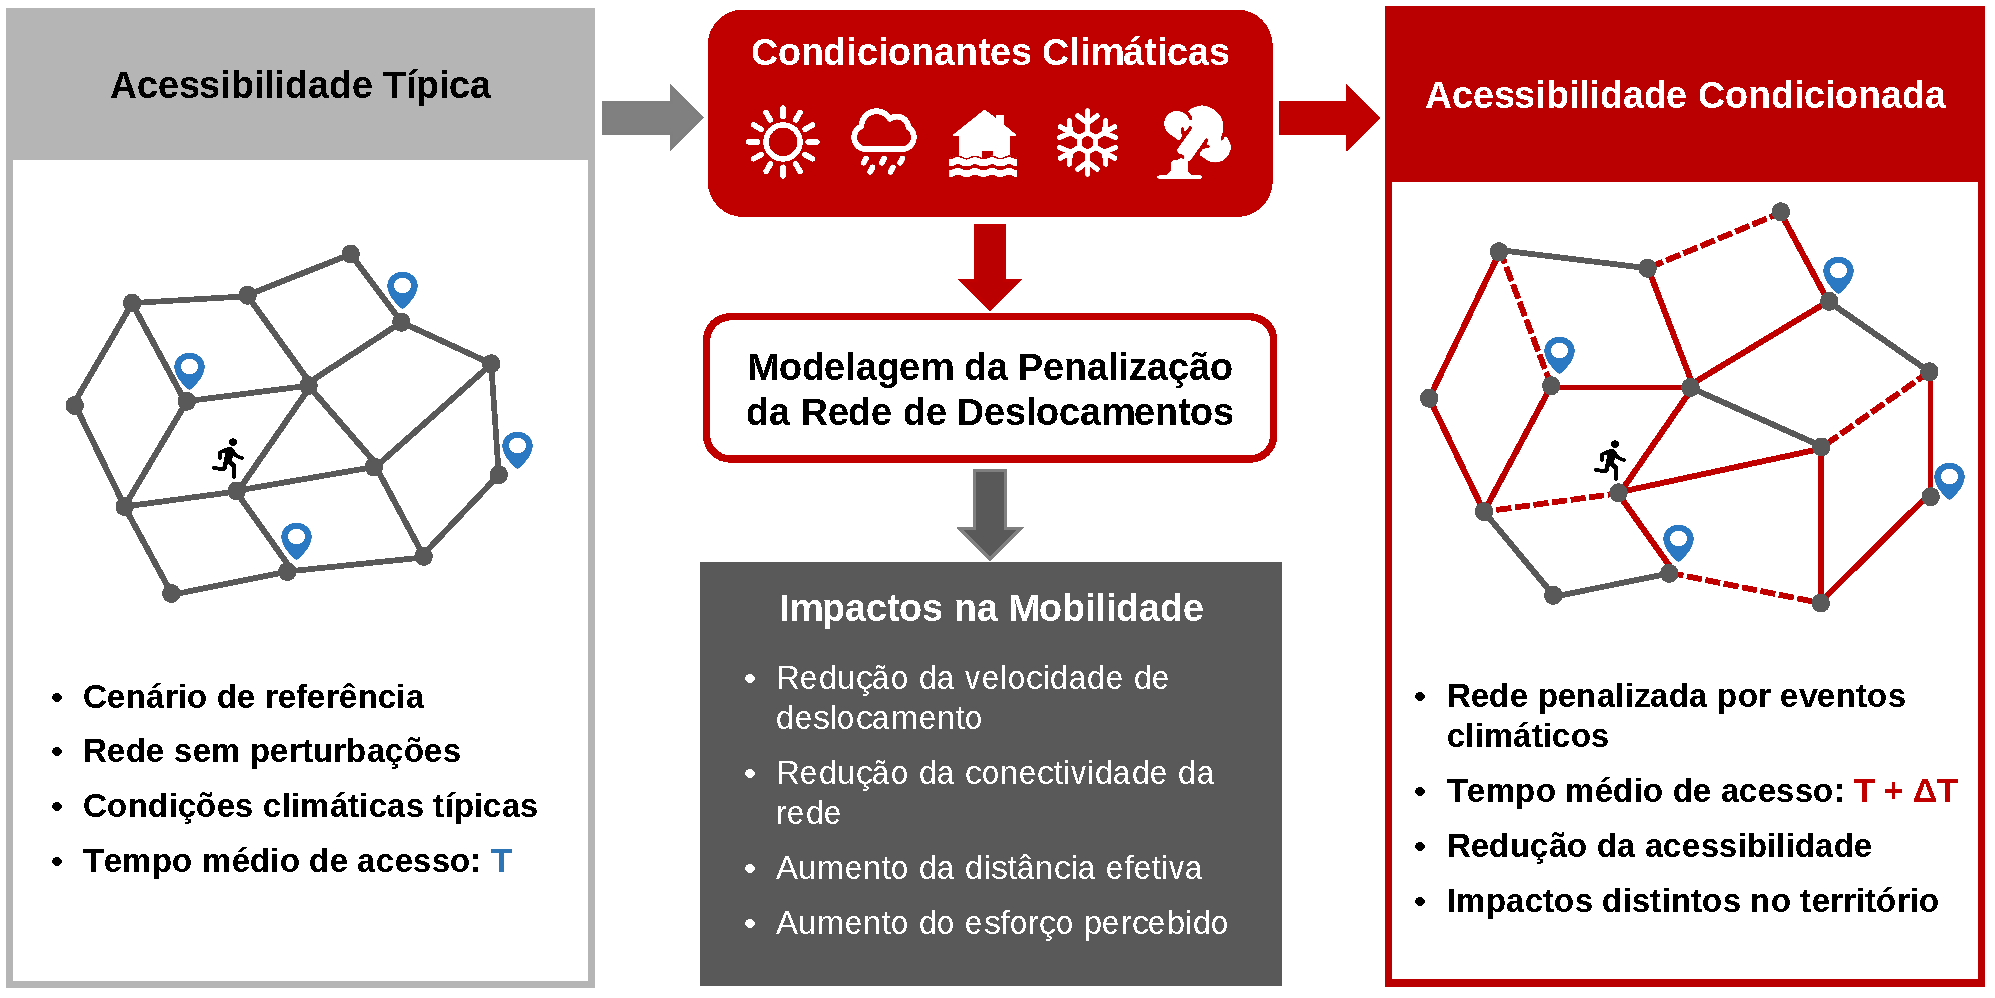
\includegraphics[width=1\textwidth]{figs/framework.pdf}
  \caption{Fluxo de modelagem dos cenários de acessibilidade. À esquerda, a rede no cenário típico, com seus custos originais de deslocamento. Ao centro, o mecanismo de penalização, que utiliza dados ambientais para penalizar a infraestrutura de mobilidade. À direita, o cenário condicionado, no qual o aumento do comprimento das arestas representa visualmente o acréscimo no tempo ou custo de deslocamento provocado pela perturbação.}
  \label{fig:framework}
\end{figure}

\subsubsection{Modelagem Territorial}
\label{subsec:territorial_modelling}

A modelagem do território urbano consiste na coleta, pré-processamento e integração de cinco camadas de dados espaciais que servem de base para a análise da acessibilidade:

\paragraph{1. Malha de análise:} Uma grade espacial regular que define a unidade mínima de estudo. A resolução da malha é ajustada ao modo de transporte e ao contexto local. O centroide de cada célula funciona como a origem teórica dos deslocamentos, servindo de base para o cálculo e a agregação dos indicadores.

\paragraph{2. Pontos de Interesse (POIs):} Representam os destinos dos deslocamentos. São coordenadas que indicam a localização dos serviços cotidianos da população, organizados em categorias (como saúde, educação e transporte). A seleção depende da disponibilidade de bases de dados locais, sejam oficiais ou colaborativas (crowdsourced).

\paragraph{3. Rede viária:} A infraestrutura de mobilidade é estruturada como um grafo espacial. Os vértices representam os cruzamentos e as arestas representam os segmentos de via, cujo peso base inicial corresponde à distância percorrida. Para possibilitar o cálculo de rotas reais, o centroide de cada célula da malha de análise é vinculado ao vértice mais próximo da rede.

\paragraph{4. Condicionantes ambientais:} Camadas espaciais, que podem ser contínuas (como imagens \textit{raster}) ou discretas (polígonos vetoriais), mapeando os fenômenos climáticos ou ambientais avaliados. Esses dados são sobrepostos à rede viária para reajustar o custo de deslocamento das arestas afetadas no cenário perturbado.

\paragraph{5. Dados Demográficos e Socioeconômicos:} Informações que caracterizam a população residente, como densidade demográfica, renda e escolaridade, oriundas de censos oficiais. Como esses dados são disponibilizados em unidades administrativas irregulares (como setores censitários), aplica-se um procedimento de compatibilização espacial para transferir o perfil socioeconômico para as células da malha regular de análise.

\subsection{O Mecanismo de Penalização e Atenuação}
\label{sec:penalization}

O framework não fixa quais variáveis ambientais devem alterar a rede, nem a
magnitude desse efeito. Ele expõe um \emph{mecanismo} que recebe camadas
ambientais e devolve um novo custo para cada aresta; a escolha das camadas e dos
parâmetros pertence a quem aplica o método. Esta seção descreve esse mecanismo.

\subsubsection{Cenários}

A rede é avaliada em dois estados. No \textbf{cenário típico}, o peso de cada
aresta ($W_{base}$) corresponde ao custo de deslocamento em condições normais —
a distância do trecho dividida pela velocidade média adotada para o modo
analisado. No \textbf{cenário condicionado}, os pesos são recalculados a partir
das camadas ambientais ($C$), produzindo $W_{cond}$ para cada aresta.

A comparação entre os dois estados é o que permite isolar o efeito da
perturbação: qualquer diferença nos indicadores de acessibilidade é atribuída à
alteração de custo introduzida pelas camadas ambientais.

\subsubsection{Modificadores de custo}

O elemento central do mecanismo é o \emph{modificador de custo}
(\texttt{CostModifier}). Cada modificador é uma função que recebe o valor de uma
camada em um ponto da aresta e devolve um fator multiplicativo:

\begin{equation}
  f(v) \rightarrow \mathbb{R}^{+}
\end{equation}

onde $v$ é o valor extraído da camada naquele ponto. O fator $f$ pode ser maior
que 1 (penalização), menor que 1 (atenuação) ou infinito (interdição). O mesmo
mecanismo cobre os três casos, e é por isso que o framework se refere a
\emph{modificadores de custo} e não apenas a penalizações.

Um modificador nunca recebe a aresta inteira: ele é aplicado a valores amostrados
ao longo dela. A forma de amostragem e a forma de agregação dos fatores são
declaradas separadamente, o que permite tratar fenômenos com distribuição
espacial distinta usando o mesmo mecanismo.

\subsubsection{Composição}

Quando mais de uma camada ambiental afeta a mesma aresta, os modificadores são
aplicados em sequência e o resultado é acumulado de forma multiplicativa:

\begin{equation}
  W_{cond} = W_{base} \times f_1 \times f_2 \times \cdots \times f_n
\end{equation}

A ordem de aplicação é declarada na configuração, e cada etapa recebe o custo
produzido pela anterior. Como a multiplicação é comutativa, a ordem não altera o
resultado numérico — mas altera como o processo é lido, o que importa quando se
quer atribuir a mudança de acessibilidade a uma camada específica.

Essa composição admite dois arranjos. Em \emph{regras simples}, cada modificador
consulta uma camada de forma independente e o encadeamento acontece entre regras.
Em \emph{regras compostas}, várias camadas são consultadas no \emph{mesmo ponto}
da aresta e o fator é calculado conjuntamente, o que permite que o efeito de uma
camada dependa do valor da outra. A distinção importa: no arranjo simples, uma
atenuação por vegetação incidiria sobre qualquer trecho arborizado, inclusive onde
não há calor algum; no arranjo composto, ela pode ser condicionada ao valor da
camada térmica no mesmo ponto.

\subsubsection{Leitura das camadas}

A forma de consultar a camada depende da natureza do dado.

\textbf{Dados contínuos} (\textit{rasters}) são amostrados em pontos ao longo da
aresta. Cada ponto recebe o valor do pixel que o contém, e os valores podem ser
lidos no ponto médio da aresta ou em vários pontos distribuídos ao longo dela. O
número de pontos é um parâmetro: mais pontos reduzem o erro em arestas longas e
heterogêneas, ao custo de mais consultas.

\textbf{Dados discretos} (polígonos vetoriais) são consultados por interseção. A
aresta é particionada nos trechos em que cruza os limites dos polígonos, e cada
trecho recebe o fator correspondente ao polígono que o contém. Trechos fora de
qualquer polígono mantêm o custo original.

\subsubsection{Agregação e interdição}

Os fatores obtidos nos pontos de uma aresta precisam ser reduzidos a um único
valor para a aresta inteira. O framework oferece duas formas:

\begin{itemize}
  \item \textbf{Máximo}: adota o fator mais restritivo observado no trecho,
    tratando a aresta pelo pior caso. É conservador e adequado quando a
    população de pontos é pequena.
  \item \textbf{Média ponderada pelo comprimento}: cada trecho paga o próprio
    fator, e a média é calculada pela extensão de cada um. É mais fiel em
    arestas longas que atravessam regiões heterogêneas.
\end{itemize}

Fatores infinitos recebem tratamento próprio. Atribuir $f = \infty$ a um trecho equivale a declará-lo intransponível: o custo de qualquer caminho que o atravesse passa a ser infinito, e o roteamento tende a preferir alternativas. A interdição não é um custo alto, mas a declaração de que a travessia não é viável naquele cenário — o tratamento adequado a fenômenos que bloqueiam a via em vez de retardá-la, como um deslizamento que soterra o trecho. Quando não existe alternativa, a célula não alcança destino algum, situação contabilizada como perda de acesso.

\subsubsection{Recálculo e indicadores}

Com os custos condicionados definidos, um algoritmo de caminho de menor custo é
executado sobre o grafo, produzindo as matrizes de tempo de viagem dos dois
cenários. A partir delas calculam-se os indicadores descritos na
Seção~\ref{sec:architecture}: o tempo médio de acesso aos $k$ POIs mais próximos
de cada categoria (PTh), a desigualdade de sua distribuição (índice G) e a fração
da população atendida dentro de um limite (F15).

A comparação entre cenários acrescenta a variação de tempo por célula e a
\emph{perda de acesso}: células que não alcançam nenhum POI no cenário
condicionado recebem tempo infinito e são contabilizadas à parte. Elas não são um
caso extremo de tempo alto — são a ausência de acesso, e tratá-las como valor
numérico distorceria qualquer média ou índice de desigualdade calculado sobre o
restante.

\subsection{Validação}
